\clearpage
\section{Exploratory data analysis}
\label{sec:eda}
The cohort diagnostics use the frozen manifest, the image inventory and the saved review decisions~[8]. We check that the retained listings have both modalities, that reviewed groups stay together and that each class has enough held-out examples to interpret its score.

\subsection{Pair quality and review decisions}
The initial audit checked 7,221 candidate image--title pairs. All candidate images decoded successfully. The review excluded five listings, yielding an acceptance rate of 99.93\%. One excluded title was in German despite its \code{en_US} tag. Four exclusions followed an inspection of the catalog type against the item shown or described, including an ottoman, a loveseat, a fabric swatch and a television media cabinet.

The audit produced 15,119 case rows. Of these, 9,177 came from title-stem matches, 4,504 from near-image matches, 1,338 from both signals and 100 from the class-stratified sample check. The review combined individual inspection and documented grouping rules.

\begin{table}[H]
\centering
\small
\caption{Outcomes for pairwise and single-listing review cases.}
\label{tab:eda-decisions}
\begin{tabular}{@{}lrl@{}}
\toprule
Decision & Count & Effect\\ \midrule
Merge & 4,813 & Link candidates into the same product group.\\
Separate & 5,999 & Require the two listings to remain in different groups.\\
Keep & 4,302 & Retain the listing or pair without adding a link.\\
Drop & 5 & Exclude a listing from the cohort.\\
\bottomrule
\end{tabular}
\end{table}

\begin{figure}[H]
\centering
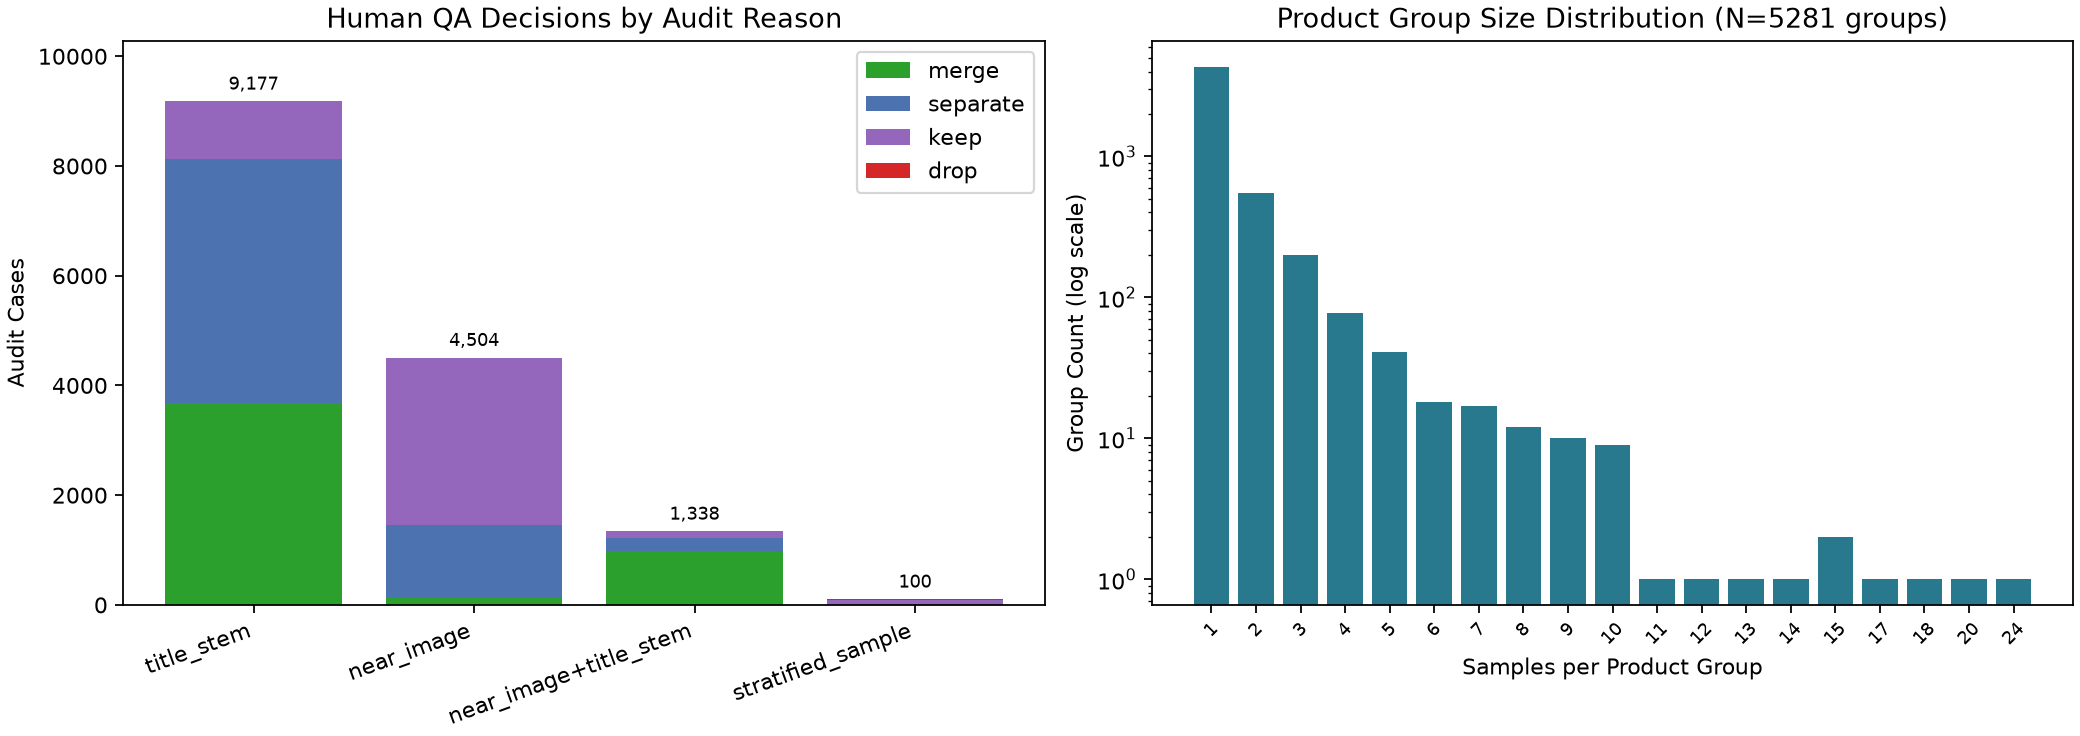
\includegraphics[width=.91\linewidth]{assets/eda/curation_and_groups.png}
\caption{Review decisions by audit reason and reviewed group sizes. The right panel uses a logarithmic frequency axis. Source: saved cohort EDA~[8].}
\label{fig:eda-curation}
\end{figure}

Figure~\ref{fig:eda-curation} shows 4,333 singletons and 948 multi-listing groups, with up to 24 items per group. After screening, no listing lacks a title or readable photo, and zero decoded-image hashes repeat.

\clearpage
\subsection{Class balance and group isolation}
The splitter targets 70/15/15 per class at seed 36, assigning whole groups. Table~\ref{tab:split} lists 5,052 training, 1,083 validation and 1,081 test listings. The 5,281 product groups divide into 3,310 train, 981 validation and 990 test groups. A direct check finds zero groups shared across splits and zero groups containing multiple catalog labels.

\begin{table}[H]
\centering
\small
\caption{Frozen membership by catalog class. Counts refer to paired listings.}
\label{tab:split}
\begin{tabular}{@{}lrrrr@{}}
\toprule
Class & Train & Validation & Test & Total\\ \midrule
\ABOSplitRows
\midrule
All classes & 5,052 & 1,083 & 1,081 & 7,216\\
\bottomrule
\end{tabular}
\end{table}

\begin{figure}[H]
\centering
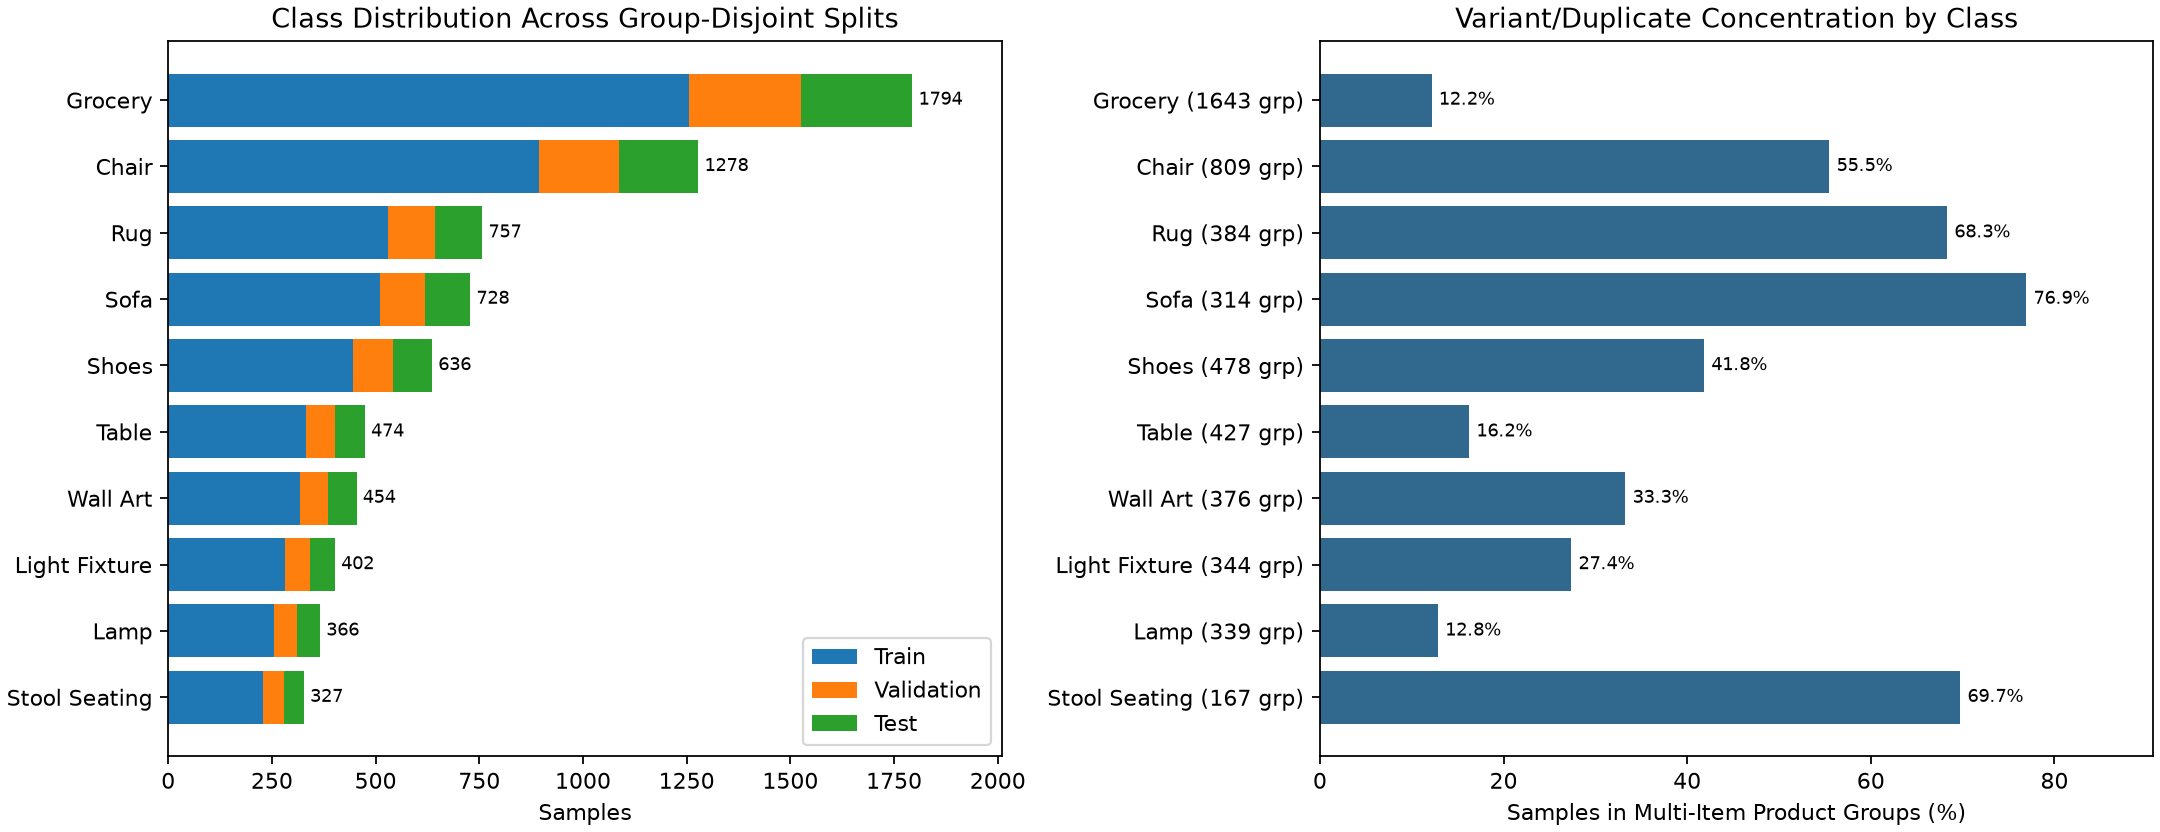
\includegraphics[width=.92\linewidth]{assets/eda/split_and_class_distribution.png}
\caption{Left: class counts by split. Right: fraction of each class in groups with multiple listings. Source: saved cohort EDA~[8].}
\label{fig:eda-split}
\end{figure}

Across the cohort, GROCERY has 1,794 listings and STOOL\_SEATING has 327, a \(5.49{:}1\) imbalance. On test they contribute 269 and 49 listings respectively. We report macro-F1 alongside accuracy so each class has equal weight in the primary metric. Multi-item groups cover 76.9\% of SOFA listings and 69.7\% of STOOL\_SEATING listings, compared with 12.2\% for GROCERY.

\clearpage
\subsection{Title length and class-name masking}
Before subword tokenization, titles contain a median of 13 whitespace-separated words, with quartiles of 10 and 16, a 95th percentile of 21 and a range of 1 to 34. The median title is 77 characters long. Table~\ref{tab:eda-title-split} tracks the small change in length between splits and the coverage of the fixed mask.

\begin{table}[H]
\centering
\small
\caption{Title length and fixed-lexicon masking by split. Percentages use the listing count in each row.}
\label{tab:eda-title-split}
\begin{tabular}{@{}lrrrr@{}}
\toprule
Split & Titles & Median words & Changed by mask & Changed (\%)\\ \midrule
Train & 5,052 & 13 & 2,365 & 46.8\\
Validation & 1,083 & 12 & 493 & 45.5\\
Test & 1,081 & 12 & 479 & 44.3\\
\midrule
All splits & 7,216 & 13 & 3,337 & 46.2\\
\bottomrule
\end{tabular}
\end{table}

\begin{figure}[H]
\centering
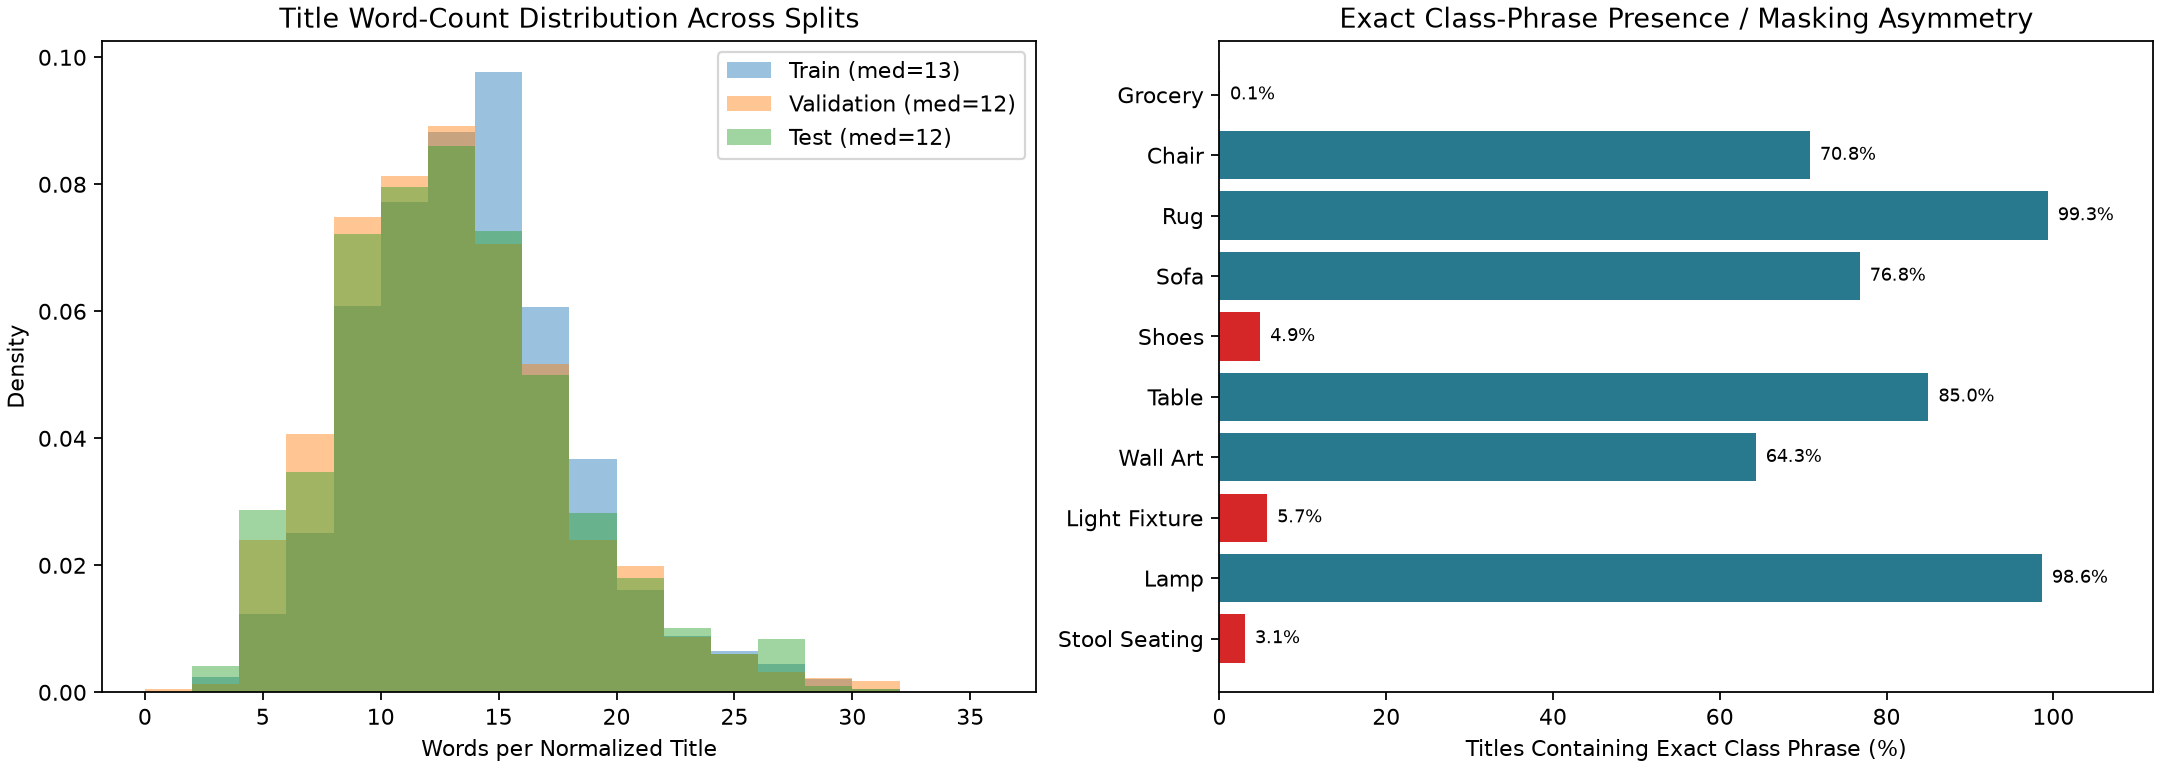
\includegraphics[width=.98\linewidth]{assets/eda/title_length_and_masking.png}
\caption{Original title length and the fraction of titles changed by an exact match to any phrase in the common class-name lexicon. The right panel groups listings by their true catalog label. Source: saved cohort EDA~[8].}
\label{fig:eda-titles}
\end{figure}

The class-name mask affects 99.3\% of RUG titles, 98.6\% of LAMP titles and 85.0\% of TABLE titles. It affects 0.1\% of GROCERY titles and 3.1\% of STOOL\_SEATING titles. A single global rule removes explicit names unevenly. For example, STOOL\_SEATING can retain related terms such as \emph{stool} and \emph{bar} when the exact phrase does not occur. This difference matters when interpreting the title baseline under the fixed policy.

\clearpage
\subsection{Photo geometry and visual context}
The JPEGs are capped at 256 pixels on the longest side. Their median width and height are both 256 pixels. The minimum width is 54 pixels and the minimum height is 36 pixels. Of the 7,216 images, 7,188 are originally RGB and 28 are grayscale. The image adapter converts all of them to RGB before resizing.

We flag a photo as extreme when its width-to-height ratio is below 0.5 or above 2.0. There are 767 such images (10.6\%). For a short-edge resize to 256 and a \(224\times224\) center crop, the retained area fraction is approximated by \((224/256)^2\min(w,h)/\max(w,h)\) for source dimensions \(w,h\). The cohort mean is 62.8\%. GROCERY and SHOES have extreme ratios on 27.0\% and 26.7\% of images respectively, with mean crop-retention estimates of 49.1\% and 50.3\%.

\begin{figure}[H]
\centering
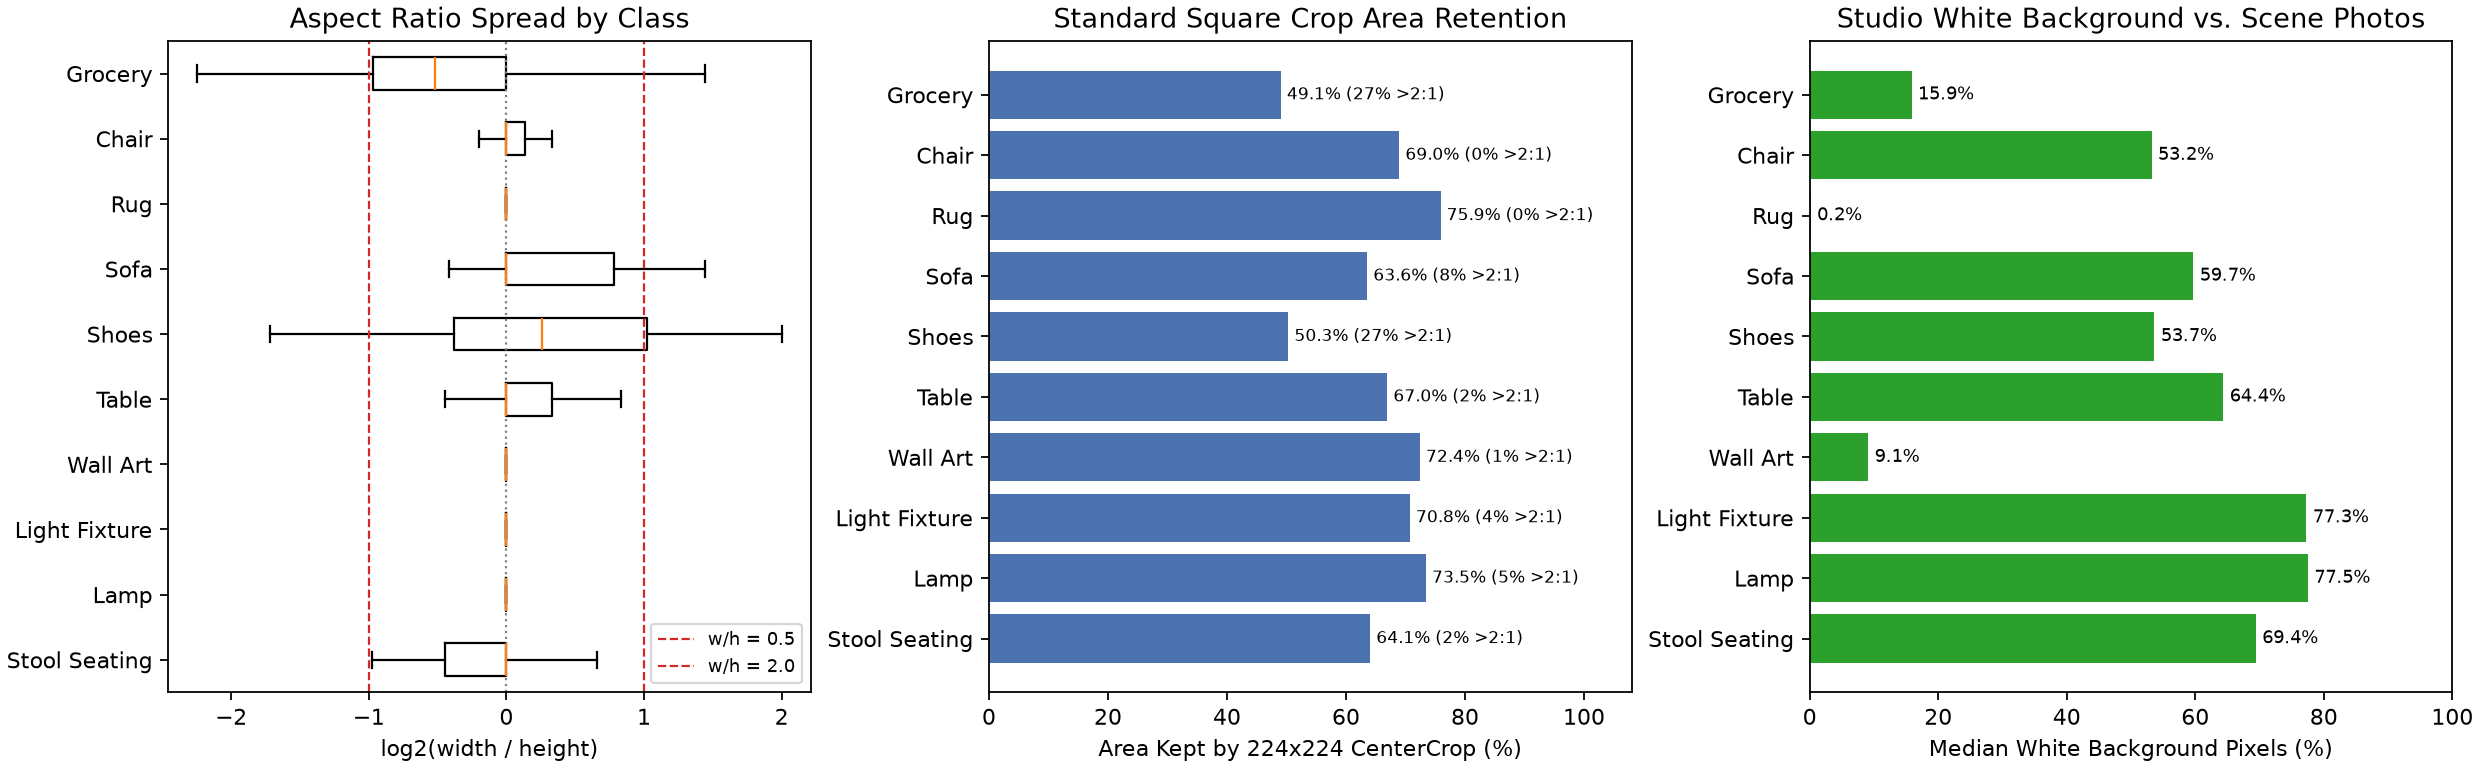
\includegraphics[width=.98\linewidth]{assets/eda/image_geometry_and_background.png}
\caption{Image aspect ratio, estimated area retained after the center crop and median near-white pixel share by class. Near-white means all three RGB channels are at least 245. Source: saved cohort EDA~[8].}
\label{fig:eda-image}
\end{figure}

The median near-white share is 77.5\% for LAMP and 77.3\% for LIGHT\_FIXTURE, compared with 0.2\% for RUG and 9.1\% for WALL\_ART. Near-white share can reflect the object itself or the image background. The geometry and pixel-space differences identify potential visual cues and show where cropping can remove substantial context. The experiment uses the same image transform for each image-based model.

\clearpage
\subsection{Repeated titles and cross-modal ambiguity}
Unicode normalization, whitespace collapse and case folding leave 106 title strings that recur across 241 listings. Of these strings, 66 occur in more than one reviewed group, 43 occur across splits, and 9 are shared by multiple catalog labels. The nine cross-label strings cover 26 listings. Group isolation preserves the reviewed product boundary while allowing titles to repeat for different items.

\begin{figure}[H]
\centering
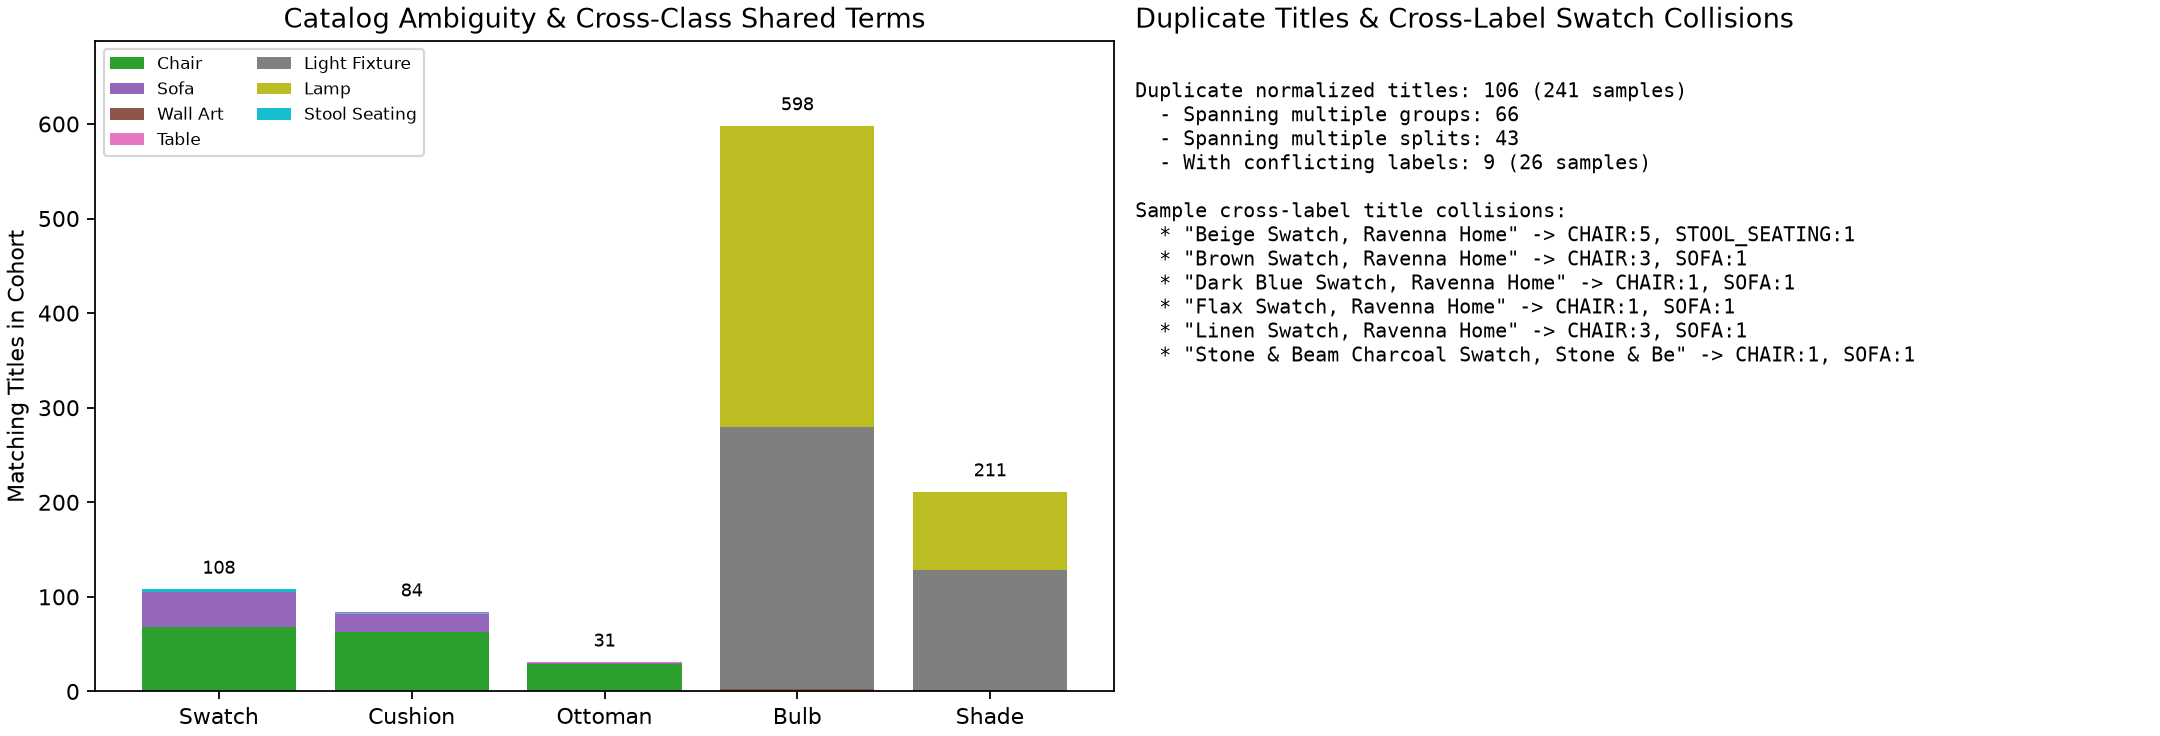
\includegraphics[width=.98\linewidth]{assets/eda/multimodal_ambiguity_and_noise.png}
\caption{Frequency of selected ambiguity terms and examples of repeated titles with different catalog labels. Counts match a term or its plural in the title. Source: saved cohort EDA~[8].}
\label{fig:eda-ambiguity}
\end{figure}

Among the seating labels, 108 listings mention \emph{swatch}, including 68 CHAIR and 37 SOFA listings. Across the cohort, \emph{bulb} appears in 598 titles, including 318 LAMP and 277 LIGHT\_FIXTURE listings. Both terms span several classes and can be ambiguous without more context.

\newcommand{\edapair}[3]{%
\begin{minipage}[t]{.153\linewidth}
\centering
\includegraphics[width=.96\linewidth,height=25mm,keepaspectratio]{assets/eda/#1.jpg}\par
{\scriptsize\textbf{#2}\par #3\par\code{#1}}
\end{minipage}}
\begin{figure}[H]
\centering
\edapair{B074MFTWGX}{Grocery}{Coconut water}\hfill
\edapair{B07Q2R4FBS}{Shoes}{Chukka boots}\hfill
\edapair{B07QF91L1T}{Lamp}{Table lamp}\hfill
\edapair{B07QGHVVHG}{Light fixture}{Flush mount}\hfill
\edapair{B07KR2S2DW}{Chair}{Dark blue swatch}\hfill
\edapair{B07KR8HR2F}{Sofa}{Dark blue swatch}
\caption{Six frozen training pairs, with shortened titles. The last two share the full title \emph{Dark Blue Swatch, Ravenna Home} and show fabric samples under different catalog labels. Photos from Amazon Berkeley Objects, CC BY 4.0~[1].}
\label{fig:eda-gallery}
\end{figure}

The gallery contrasts useful agreement, such as the chukka boot image and title, with paired swatches that show and describe fabric. The seating type is difficult to recover from the latter pair because neither input depicts the catalog object.

\clearpage
\subsection{Residual cues in training titles}
We inspected brand metadata and residual terms on the training split. Of 5,052 training listings, 5,051 have a recorded brand across 76 distinct brand strings. A brand's dominant-class share is the fraction of its listings assigned to its most common class. Table~\ref{tab:eda-brands} contrasts broad furniture brands with brands whose sampled products concentrate in one class.

\begin{table}[H]
\centering
\small
\caption{Selected brand--label associations measured on train only.}
\label{tab:eda-brands}
\begin{tabular}{@{}lrrlr@{}}
\toprule
Brand & Listings & Classes & Dominant class & Share\\ \midrule
Stone \& Beam & 1,253 & 8 & CHAIR & 26.6\%\\
Rivet & 1,231 & 8 & CHAIR & 21.2\%\\
365 by Whole Foods Market & 427 & 1 & GROCERY & 100.0\%\\
find. & 198 & 1 & SHOES & 100.0\%\\
\bottomrule
\end{tabular}
\end{table}

\begin{figure}[H]
\centering
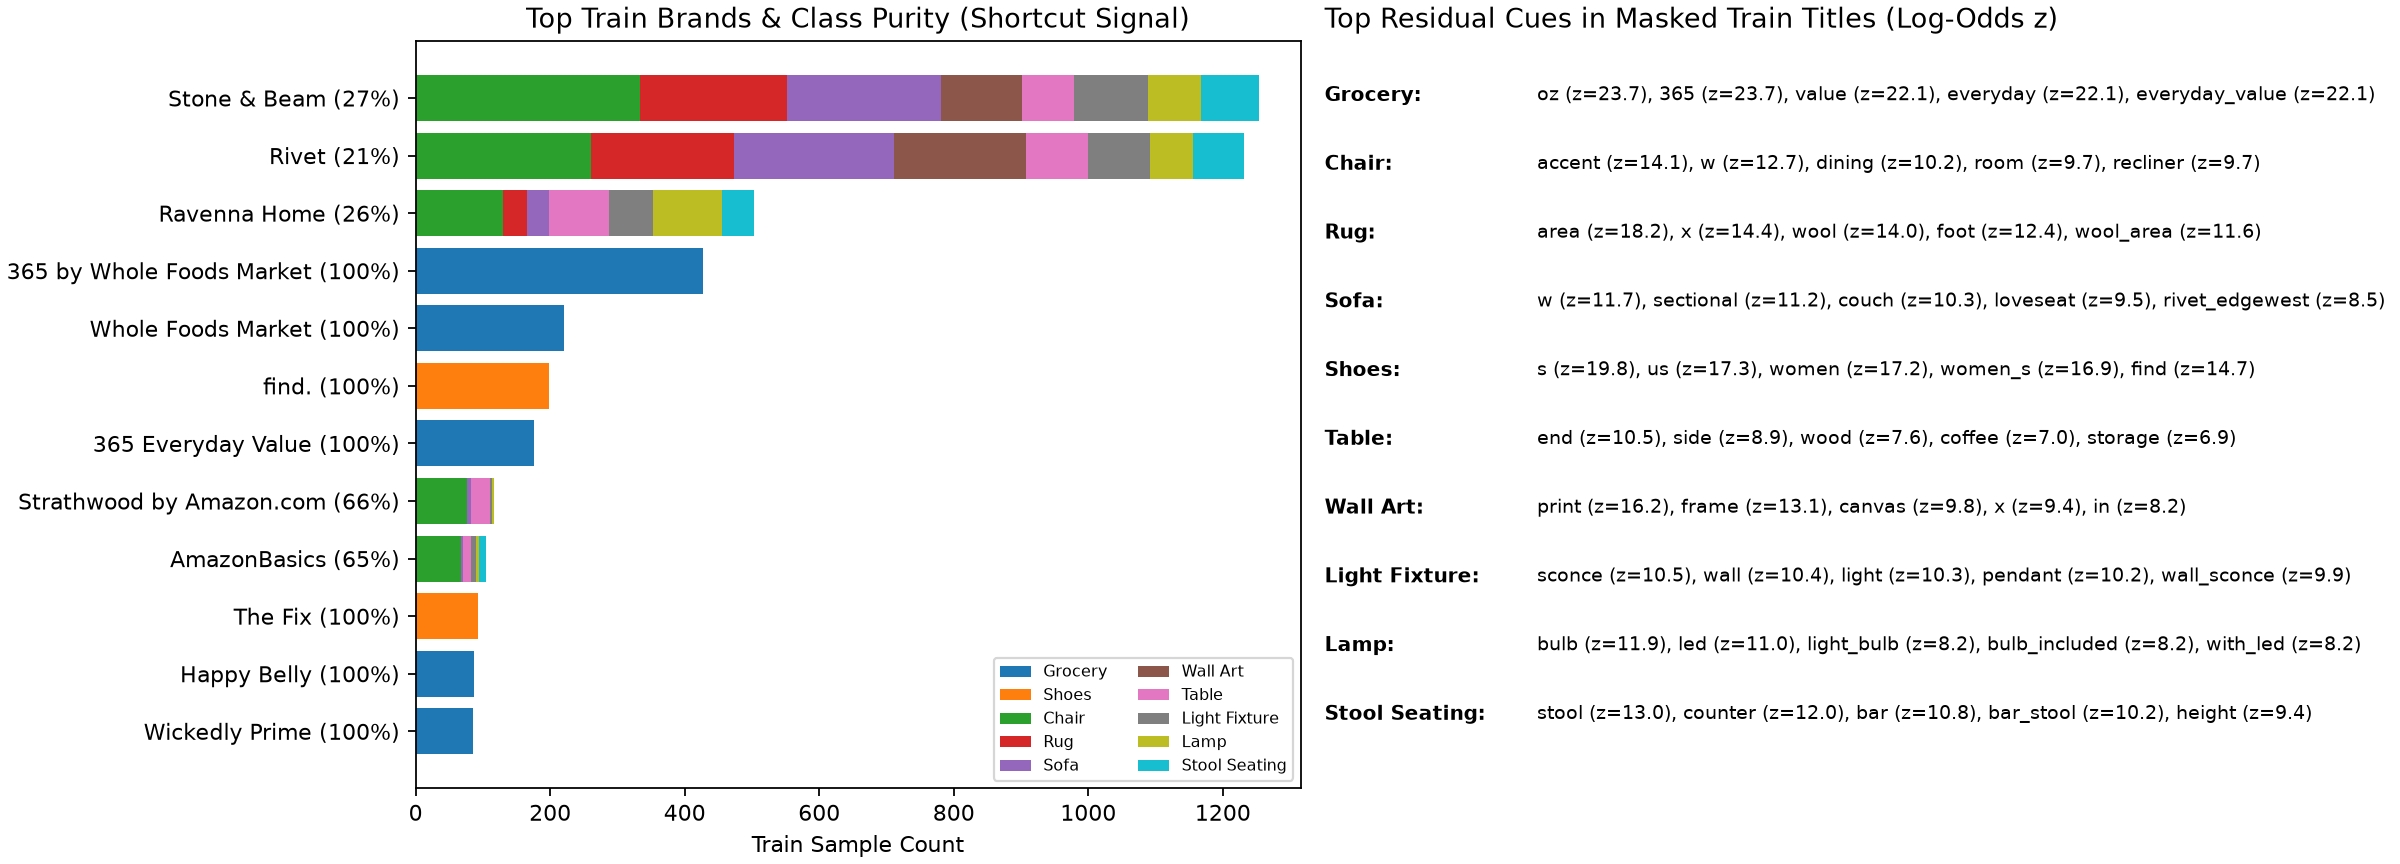
\includegraphics[width=.98\linewidth]{assets/eda/train_brand_and_lexical_cues.png}
\caption{Brand composition and residual word and phrase associations in masked training titles. The latter are ranked by smoothed log-odds relative to the other classes. Source: saved cohort EDA~[8].}
\label{fig:eda-lexical}
\end{figure}

After masking, \code{oz} occurs in 638 training titles and \code{365} in 636, all in GROCERY. \code{sconce} occurs in 109 training titles, 107 with label LIGHT\_FIXTURE. The model receives the title string, which can contain brand names or related terms. The separate brand metadata field is used in this diagnostic. These observations document associations that remain after masking and should be considered when assessing generalization to other catalogs.

